\section{Software Process Evaluation from User Perceptions and Log Data}
\label{sec:combining-questionnaier-and-trace}

%\todo[inline]{Damjan work. This work is to better understand resources. Do we need to put a subjective perspective in this thesis?}

This section proposes a new approach that combines two different perspectives on the same phenomenon. We apply our methods in the context of our industry partner, an Austrian \gls{sme} which offers document management software solutions. We conducted mixed-method research. First, a questionnaire is used to gather user-subjective information from domain experts on specific items. Second, trace data are used which provide the ground truth to objectively analyze those items. Finally, inductive reasoning is used to draw conclusions and suggest recommendations. The following sections describe the approach itself and its results on a case study from an industry partner. 

\subsection{Combined Approach for Evaluating the Software Process}

The proposed approach builds on established SDM evaluation approaches. However, unlike existing approaches that base their SDM evaluation on stakeholder perceptions, the proposed approach complements stakeholder perceptions with data from development tools’ logs. An overview of the approach is shown in \Cref{fig:sdm-process}. Let us now describe each step of the process.

\begin{figure}
	\centering
	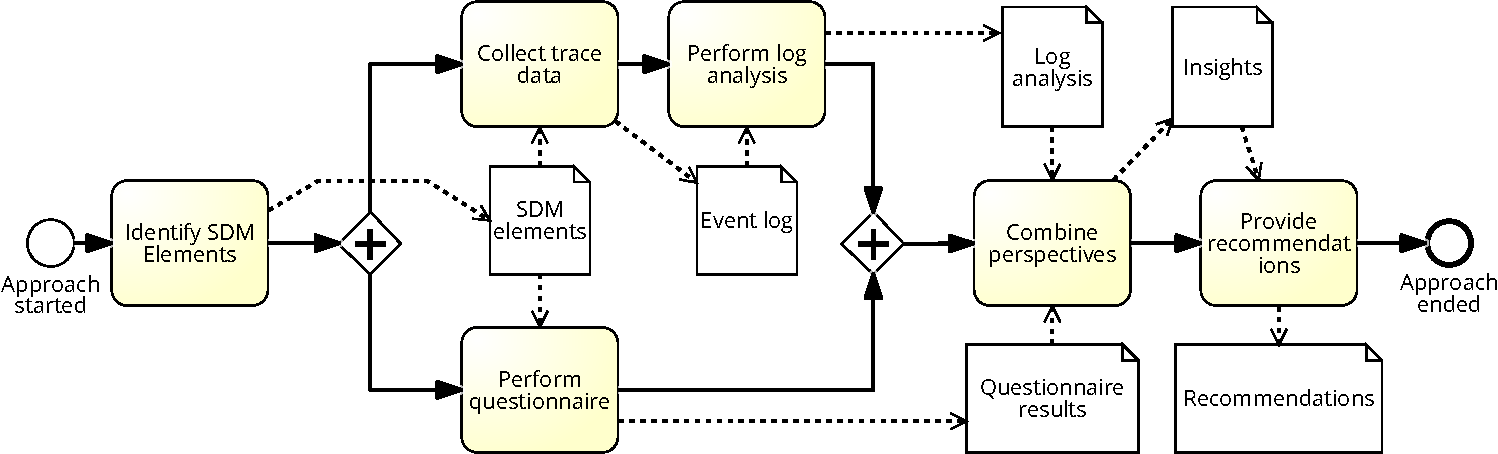
\includegraphics[width=\linewidth]{figures/SDM-process}
	\caption[Combined evaluation of trace and questionnaire data]{Combined evaluation of trace and questionnaire data in software development}
	\label{fig:sdm-process}
\end{figure}

\begin{inparadesc}
	\item[\bfseries Identification of SDM elements.] In this phase \gls{sdm} elements for evaluation are first identified and catalogued with the help of key stakeholders knowledgeable about their SDM (e.g. process managers, project managers, senior developers). After the SDM elements are catalogued the management has to identify the stakeholders importantly affected by specific SDM elements. This means that developers who perform certain SDM activity should be the ones to evaluate this SDM activity from a developer perspective. Likewise, managers responsible for certain SDM activity should be the ones to evaluate this SDM activity from managerial perspective. Similar logic is applied also to other stakeholders importantly affected by specific SDM elements. \\
	
	\item[\bfseries Perform questionnaire.] This activity starts starts with the creation of questionnaires based on the predefined template questions that are used to create more specific questions for each SDM element cataloged in the identification phase. Such questionnaire are answered by the stakeholders of the process. Subsequently, their results are collected and made available for further analyses. \\
	
	\item[\bfseries Collect Trace Data.] For each \gls{sdm} element, trace data are collected from information systems logs. This is a challenging task as organizations may adopt a multitude of tools to support their process. Typical tools include issue-trackers (e.g., Bugzilla, Microsoft Dynamics CRM), continuous integration (CI) managers (e.g. Jenkins), project management tools (e.g., Asana, JIRA), version control systems (Git, Subversion), and many more. 
	
	In the context of this we collected event logs from Jira from our industry. These event logs contain information about the users who worked in various tasks such as bug fixing, feature specification, and implementation. Considering the information gathered from the questionnaire, we noticed that these tasks represent elements on which were perceived differently from management and developers. As an example, bug was perceived as critical element by developers but was ranked low by managers. Thus, a dissonance of perceptions was in place. In this case, facts recorded in event logs such as time spent on bugs and productivity provide a further dimension for understanding the gap between perception and actual importance of the element. The output of this step is an event log. \\
	
	\item[\bfseries Perform Log Analysis.] The input of this phase is an event log. It applies process mining on the event logs, taking into account the mapping of the event log to the activities provided in the previous step. In order to perform this step, the event log may be sliced and filtered into several sub-logs, depending on the aspect of reality which is intended to be analyzed. As a result, several insights in the form of process models and statics are made available for further analysis. \\
	
	\item[\bfseries Combine perspectives and Provide Recommendations.] After the event logs have been analyzed, a 
	 The input of this phase is an event log. It applies process mining on the event logs, taking into account the mapping of the event log to the activities provided in the previous step. In order to perform this step, the event log may be sliced and filtered into several sub-logs, depending on the aspect of reality which is intended to be analyzed. As a result, several insights in the form of process models and statics are made available for furtherThese insights are further used to analysis by the user. These insights, combined with the information from the questionnaire, can be used to provide recommendations (e.g., \emph{Element X is perceived as useful but it makes developers less efficient}).
	
\end{inparadesc}



%\todo[inline]{Start working from here.}
%
%\paragraph{\bfseries Collect Trace Data}
%
%For each \gls{sdm} element, trace data are collected from information systems logs. This is a challenging task as organizations may adopt a multitude of tools to support their process. Typical tools include issue-trackers (e.g., Bugzilla, Microsoft Dynamics CRM), continuous integration (CI) managers (e.g. Jenkins), project management tools (e.g., Asana, JIRA), version control systems (Git, Subversion), and many more. 
%
%In the context of this we collected event logs from Jira from our industry. These event logs contain information about the users who worked in various tasks such as bug fixing, feature specification, and implementation. Considering the information gathered from the questionnaire, we noticed that these tasks represent elements on which were perceived differently from management and developers. As an example, bug was perceived as critical element by developers but was ranked low by managers. Thus, a dissonance of perceptions was in place. In this case, facts recorded in event logs such as time spent on bugs and productivity provide a further dimension for understanding the gap between perception and actual importance of the element. 
%
%\paragraph{Phase 4 – Recommendations}
%
%This phase is concerned with the development of recommendations for improvements. Specifically, the results from the previous phase are analyzed and put into context. Particular attention is paid to outliers. For instance, significant deviations from Agile guidelines, might be a bad practice to follow. Recommendations would pinpoint such cases.  

\subsection{Case Study}

The proposed approach was tested in an Austrian \gls{sme} software development company located in Vienna. The company can be considered a typical central European \gls{sme}. The company develops software products for the field of Customer Communication Management paying special attention to the areas of document composition, workflow and document distribution. Their customers come from eight different central and southern European countries. 

A single case study design was employed to assess the proposed approach. Such design is appropriate when it captures the circumstances and conditions of an everyday or commonplace situation \citep{yin2017case}. The studied company represents a typical \gls{sme} in the software development industry. To collect the data, we conducted interviews with management and process engineer, directly observed their workday, surveyed all the employees involved in company’s software development process and collected software development tool logs. 

All participants of our study were experienced developers having worked as members of the same team for at least two years. 

In the following, after having identified the key \gls{sdm} elements with the help of domain experts, we divide the process from \Cref{fig:sdm-process} in three phases: 
\begin{inparaenum}[\itshape i)]
	\item conducting the survey;
	\item performing log analysis; and
	\item combining the outcomes.
\end{inparaenum}

\subsubsection{Conducting the Survey}

Different questionnaires are created for each stakeholder based on the predefined template questions. In line with the established measures from studies presented in the literature review the developers report their perceptions about their use and satisfaction concerning a certain SDM element. Similarly, management reports their perceptions about SDM impact on iron triangle measures of overall project success (cost, speed and quality) and process engineers report their perceptions about SDM element level of assimilation, relative advantage and compatibility. The questions are written in form of statements where answers are given on 7-point Likert scale. The template statements are presented in \Cref{fig:surveymethod}. 

\begin{figure}
	\centering
	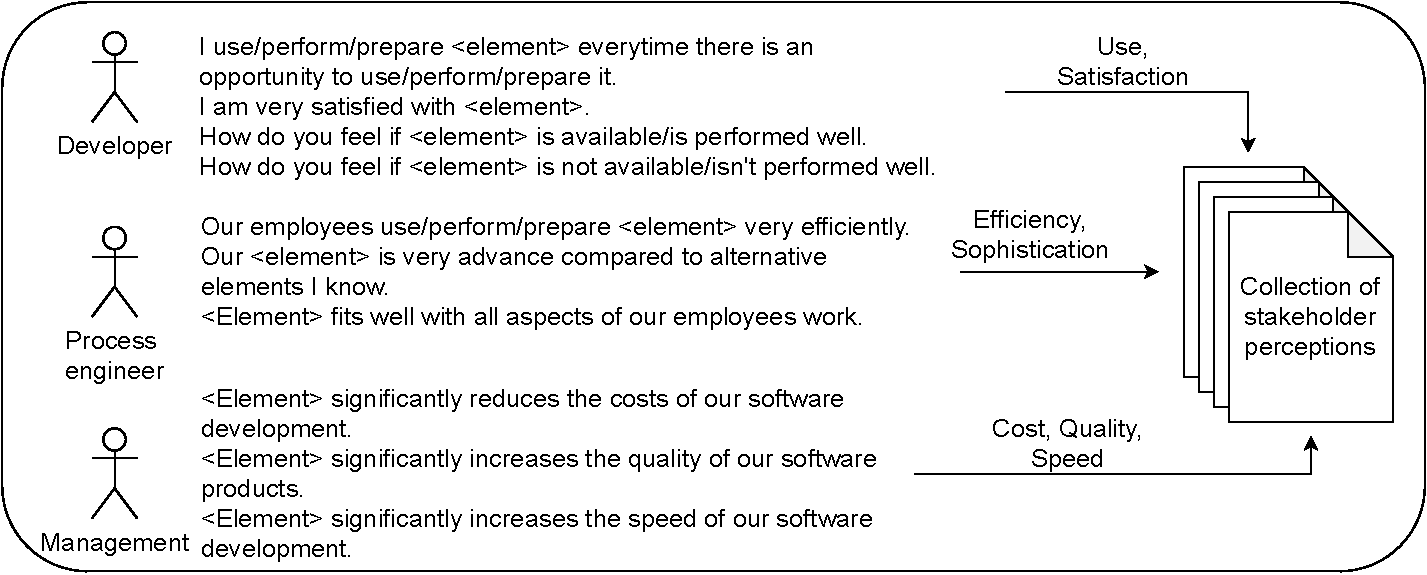
\includegraphics[width=\linewidth]{figures/SurveyMethod}
	\caption[Survey templates used for gathering stakeholders perceptions]{Template for survey and analysis of stakeholder perceptions of SDM elements}
	\label{fig:surveymethod}
\end{figure}

To analyze stakeholder perceptions, we position SDM elements in a multidimensional space based on the average measurement of each stakeholder perception (dimension). It is typically difficult to further improve SDM elements that are considered highly beneficial by all stakeholders since they are all already satisfied with them. On the contrary, SDM elements that are considered unbeneficial by all stakeholders have high potential for improvement, since it is likely that most stakeholders will support their change. The SDM elements where perceptions of stakeholders greatly differ require further examination where log analysis has an important role to identify appropriate improvement actions.

For the purpose of analysis, we visualize perceptions of two different stakeholders on a scatter chart. \Cref{fig:survey-scatter-plot} reports the results of the survey. In the x-axis (User) are reported the perception scores of the developers, in the y-axis (Process) are reported the perceptions of process engineers, colors represent the perceptions of management (green is high).


\begin{figure}
	\centering
	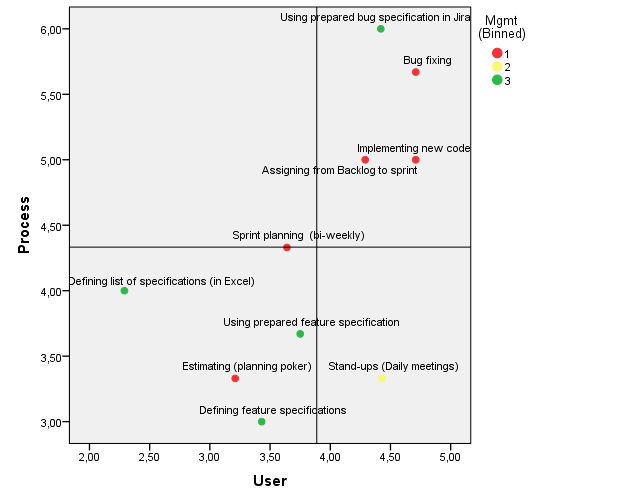
\includegraphics[width=\linewidth]{figures/survey-scatter-plot}
	\caption[Survey results on user perceptions]{Results of questionnaire about the perceptions of stakeholders about the identified SDM elements}
	\label{fig:survey-scatter-plot}
\end{figure}

This chart helps us to detect activities to investigate further with log analysis. Detailed analysis was performed on the activities: \emph{Bug fixing}, \emph{Implementing new code}, \emph{Assigning from backlog to sprint}, and \emph{Sprint planning}. We selected these activities based on conflicting stakeholder perceptions and availability of log data. Especially, the activities are characterized by either by low management perception and relatively high developers and process engineer perceptions or by high management perception and low developers and process engineer perceptions (e.g., \emph{Defining feature specifications}).

\subsubsection{Performing log analysis}

The company uses the JIRA issue tracking software to keep change of the various tasks being performed by the employees. Employees in this case are software engineers and developers. We collected all activities done by employees during the time period between the dates 2015-12-30 and 2017-05-16.  The JIRA log was further preprocessed to generate various tabular datasets and event logs that can be used by process mining tools. For what concerns the tabular datasets, we created specific attributes to keep count of the different activities performed. Focus activities were bug fixing, implementing new code and feature specification. As typical tasks in software engineering projects are part of sprints, we aggregated the information into two-week intervals. This helps us to shed light into tasks that were delayed or dragged along slowly. Furthermore, we kept included in our dataset the users who performed the various activities.  

The output of this phase is to create an event log and analyze. To this end, we inspected manually all the event logs that contain information about the \gls{sdm} elements that we could obtain from our industry partner. Collected logs were unstructured or not ready to be analyzed. Therefore, a preprocessing step was required in order to transform these logs into a format which can be further analyzed by process mining techniques. More specifically, the data was transformed into a tabular format such a CSV. Out of the columns, we manually identified the three attributes required for process mining: case (i.e., which instance of the process is stored), activity (what activity is done in the instance), and timestamp (when is an activity performed). More specifically, with reference to the attributes from JIRA, we considered \emph{project identifier} as case id, the field \emph{typeText} (e.g., Bug, Feature, Improvement, etc) as activity type, \emph{assigneeUserName} as the human resource who did the task, and the fields \emph{created}, \emph{updated} and \emph{resolved} as timestamps. The other attributes present in the log, we used as auxiliary fields to perform more detailed analyses such as filtering of a particular resource, project and select only completed tasks. As a last step, we anonymized the event log by mapping the resource names to distinct symbols $p_1, ... p_n$.


For what concerns process mining event logs, we did not apply any aggregation as different process mining techniques work with different levels of granularity. Thus, we focused on generating event logs for respectively bug fixing, implementing new code and feature specification. As a results we obtained XES files which are the input of our analyses from a process perspective. 

Chosen elements were performed by six different resources. Such resources are reported anonymously as p1, p2, p3, p4, p5, p6. Some tasks were completed in the system without being assigned to any resource. To capture this, we included a special resource named “no resource”.  

We then imported the different event logs in the Disco tool for process mining and computed the efficiency of task burn-down by different users. In the following we report on this results and interpret them against the perceptions from the questionnaire.

\subsubsection{Combining perceptions and log analyses}

This phase provides insights on the performance of resources regarding the selected activities.  We analyzed the overall level of activity done by resources.  Our analyses showed that the activities of bug fixing and implementing new code were done according to sprints. One Sprint is considered as fourteen days, i.e., two full weeks including weekends. Table 1 shows the overall activity done in the first three sprints. More specifically, Sprint 1 refers to the amount of activity done in the first fourteen-day period. Sprint 2 refers to the second fourteen-day timeslot. Sprint 3 refers to the third fourteen-day period. Additionally, the count the number of activities performed beyond the sprints. Especially, we are interested in the amount of activities completed by a resource than three sprints.  

\Cref{tab:outcome} summarizes the results of these results for bug-fixing, which scored high in developers and engineers perceptions but low in the managers perception. We organize the table by Sprint (i.e., the considered time windows). Column Activities represents how many times was activity performed by certain person on this project.

% Please add the following required packages to your document preamble:
% \usepackage{booktabs}
% \usepackage{graphicx}
\begin{table}[]
	\centering
	\caption{Outcome of the process mining analyses}
	\label{tab:outcome}
	\resizebox{!}{!}{%
		\begin{tabular}{@{}crrrrrrrrrr@{}}
			\toprule
			&
			\multicolumn{2}{c}{Sprint 1} &
			\multicolumn{2}{c}{Sprint 2} &
			\multicolumn{2}{c}{Sprint 3} &
			\multicolumn{2}{p{1.5cm}}{Sprint: all except first three} &
			\multicolumn{2}{c}{Total} \\ \midrule
			Resource &
			\multicolumn{2}{c}{Activities} &
			\multicolumn{2}{c}{Activities} &
			\multicolumn{2}{c}{Activities} &
			\multicolumn{2}{c}{Activities} &
			\multicolumn{2}{c}{} \\ \cmidrule(lr){2-9}
			p1         & 18  & 13.24\%  & 6  & 20.69\%  & 4  & 15.38\%  & 10 & 38.46\%  & 52  & 19.33\%  \\
			p2         & 51  & 37.50\%  & 8  & 27.59\%  & 10 & 38.46\%  & 8  & 30.77\%  & 95  & 35.32\%  \\
			p3         & 67  & 49.26\%  & 15 & 51.72\%  & 12 & 46.16\%  & 8  & 30.77\%  & 122 & 45.35\%  \\
			Tot Sprint & 136 & 100.00\% & 29 & 100.00\% & 26 & 100.00\% & 26 & 100.00\% & 269 & 100.00\% \\ \bottomrule
		\end{tabular}%
	}
\end{table}

We analyzed the performance of resources who work on bug fixing for a specific project. In order to compare the performance of the various resources, we considered their percentage of work over the total number of items completed in each sprint. That is, resource p1 has completed 13.24\% of the overall tasks that were completed in Sprint 1. This is an indicator of the share of work this resource has contributed with. Furthermore, p1 has completed relatively more tasks with delay. This information is visible under column ``Sprint: all except first three''. In this case, we observe 38.46\%. Thus, we can notice that p1 is underperforming in context of the analyzed project for the task of bug fixing. 

Bug-fixing was the most demanding activity. Resource p1, p2, and p3 were active on this element, whereas resource p4, p5 and p6 were only seldom involved as their share of tasks is significantly lower than the previous three resources. Thus, we do not report their frequencies in this table. Out the active resources on this element, p1 is clearly underperforming. In fact, its completed tasks amount to less than one third of the tasks completed by p3, who appears to be the top performer. Furthermore, column "Sprint: all except first three´´ indicates that resource p1 is dragging tasks along sprints and its backlog keeps growing. 

With these results at hand, we can look back at the questionnaire and compare the questions answered by each resource. For example, we can observe that some resources have stated that the specific element (e.g., bug-fixing) improves their speed. However, event log analyses showed a growing backlog of tasks. Therefore, we are able to pinpoint a dissonance between perceptions and reality. Such dissonance should be resolved by further analysis on the quality of the tasks themselves. Specifically, domain experts should use our results as a staring point to verify whether certain elements which are perceived positively are actually useful for the organization. At the same time, attention must be paid to find the reasons of underperformance. To this end, a more qualitative analysis is necessary in order to understand whether the poor performance is associated to the tool or to the complexity of the task itself.  

